\documentclass[a4paper,12pt,openany,oneside]{book}

% 字体配置文件
% !TEX TS-program = XeLaTeX
% !TEX encoding = UTF-8 Unicode

% 英文字体设置特别推荐方案(Windows,需要安装 Adobe 字体),现代
% \usepackage[UTF8]{ctex}
\usepackage{fontspec}
\usepackage{xltxtra,xunicode}
\usepackage[CJKnumber,CJKchecksingle,BoldFont]{xeCJK}
\usepackage{amsmath}
\usepackage{amssymb}
\setmainfont[Mapping=tex-text]{Times New Roman}
\setsansfont[Mapping=tex-text]{Arial}
% \newfontfamily\tempus{FandolSong}
\newfontfamily\tempus{SIMSUN.TTC}  % 如果这里编译错误,请自行替换为系统中的宋体字体名
% \newfontfamily\ms{MS Sans Serif}
%\setmonofont{Consolas}


% 英文字体设置方案一(Windows,需要安装 LM10 字体),和 LaTeX 默认字体保持一致,经典
% \usepackage{amssymb}
% \usepackage{fontspec}
% \usepackage{amsmath}
% \usepackage[CJKnumber,CJKaddspaces,CJKchecksingle,BoldFont]{xeCJK}
% \usepackage{mathrsfs}   % 一种常用于定义泛函算子的花体字母,只有大写。
% \usepackage{bm}         % 处理数学公式中的黑斜体的宏包
% \setmainfont{LMRoman10-Regular}
% \setsansfont{LMSans10-Regular}
% \setmonofont{LMMono10-Regular}

% 英文字体设置方案二(Linux,使用自带 LM10 字体),和 LaTeX 默认字体保持一致,经典
% \usepackage{fontspec}
% \usepackage{amsmath,amssymb}
% \usepackage[CJKnumber,CJKaddspaces,CJKchecksingle,BoldFont]{xeCJK}
% \usepackage{mathrsfs}   % 一种常用于定义泛函算子的花体字母,只有大写。
% \usepackage{bm}         % 处理数学公式中的黑斜体的宏包
% \setmainfont{LMRoman10}
% \setsansfont{LMSans10}
% \setmonofont{LMMono10}

% 英文字体设置方案三(Linux,使用自带 Nimbus 字体),和 Word 模版字体保持一致,经典
% \usepackage{fontspec}
% \usepackage{mathptmx}
% \usepackage{amsmath,amssymb}
% \usepackage[CJKnumber,CJKaddspaces,CJKchecksingle,BoldFont]{xeCJK}
% \usepackage{mathrsfs}   % 一种常用于定义泛函算子的花体字母,只有大写。
% \usepackage{bm}         % 处理数学公式中的黑斜体的宏包
% \setmainfont{Nimbus Roman No9 L}
% \setsansfont{Nimbus Sans L}
% \setmonofont{Nimbus Mono L}

% 中文字体设置,使用的是 Adobe 字体,保证了在 Adobe Reader / Acrobat 下优秀的显示效果
\setCJKmainfont[BoldFont={SIMSUN.TTC},ItalicFont={SIMSUN.TTC}]{SIMSUN.TTC}
\setCJKsansfont{SIMHEI.TTF}
\setCJKmonofont{SIMSUN.TTC}
% \setCJKmainfont[BoldFont={FandolSong},ItalicFont={FandolSong}]{FandolSong}
% \setCJKsansfont{FandolHei}
% \setCJKmonofont{FandolSong}

% 定义字体名称,可在此添加自定义的字体
\setCJKfamilyfont{song}{SIMSUN.TTC}
\setCJKfamilyfont{hei}{SIMHEI.TTF}
\setCJKfamilyfont{hwxhei}{STXIHEI.TTF}
\setCJKfamilyfont{hwxkai}{STXINGKA.TTF}
% \setCJKfamilyfont{song}{FandolSong}
% \setCJKfamilyfont{hei}{FandolHei}
% \setCJKfamilyfont{hwxhei}{FandolHei}
% \setCJKfamilyfont{hwxkai}{FandolKai}
% \setCJKfamilyfont{FandolHei}{STXihei} 
% \setCJKfamilyfont{FandolKai}{华文行楷}
% \setCJKfamilyfont{FandolHei}[AutoFakeBold = {2.17}]{华文细黑}
%\setCJKfamilyfont{fs}{Adobe Fangsong Std}
%\setCJKfamilyfont{xkai}{STXingkaiSC-Bold}

% 自动调整中英文之间的空白
% \punctstyle{quanjiao}
\XeTeXlinebreaklocale "zh"      %中文断行
\XeTeXlinebreakskip = 0pt plus 1pt %1pt左右弹性间距

% 其他字体宏包


% 宏包配置文件
% !TEX TS-program = XeLaTeX
% !TEX encoding = UTF-8 Unicode

%%%%%%%%%%%%%%%%%%%%%%%%%%%%%%%%%%%%%%%%%%%%%%%%%%%%%%%%%%%%%%%%%%%%%% 
% 
%	大连理工大学本科生毕业设计(论文)LaTeX 模版 —— 格式文件 format.tex
%	版本:1.0
%	最后更新:2022.5.12
%  	修改者:赵小棠 (E-amil: xiaotang_zhao@outllook.com)
%	编译环境:win10 TeXstudio textlive2020 编译器XeLaTeX
% 
%%%%%%%%%%%%%%%%%%%%%%%%%%%%%%%%%%%%%%%%%%%%%%%%%%%%%%%%%%%%%%%%%%%%%% 

% 页面设置
\usepackage[body={16.1cm, 22.2cm}]{geometry}
\usepackage{indentfirst}                         % 首行缩进宏包
\usepackage[sf]{titlesec}                        % 控制标题的宏包
\usepackage{titletoc}                            % 控制目录的宏包
\usepackage{fancyhdr}                            % 自定义页眉页脚
\usepackage{fancyref}                            % 引用链接属性
\usepackage[perpage,symbol]{footmisc}            % 脚注控制
\usepackage{layouts}                             % 打印当前页面格式的宏包
\usepackage{paralist}                            % 一种换行不缩进的列表格式,asparaenum,inparaenum 等
\usepackage[shortlabels]{enumitem}               % 列表格式
\usepackage{fancyvrb}                            % 原样输出
\usepackage[amsmath,thmmarks,hyperref]{ntheorem} % 定理类环境宏包
\usepackage{type1cm}                             % 控制字体的大小

% 表格处理
\usepackage{booktabs}   % 三线表
\usepackage{multirow}   % 表格多行处理
\usepackage{diagbox}    % 斜线表头
\usepackage{tabularx}   % 表格折行
\usepackage{siunitx}    % 国际单位,小数点对齐


% 图形相关
\usepackage{graphicx}         % 请在引用图片时务必给出后缀名
\usepackage{caption}				 % 浮动体添加标题
\usepackage[x11names]{xcolor} % 支持彩色
\usepackage{placeins}  % 浮动图形控制宏包
\usepackage{rotating}	      % 图形和表格的控制
\usepackage{picinpar}
\usepackage{setspace}         % 定制表格和图形的多行标题行距
\usepackage{subfigure}           % 插入子图形
% \usepackage{subcaption}

\usepackage{listings}         % 源代码展示
\lstset{%
  language=TeX,
  defaultdialect=empty,
  basicstyle=\ttfamily\small,
  backgroundcolor=\color{LightSteelBlue1},
  keywordstyle=\color{blue},
  showspaces=false,
  showstringspaces=false,
  showtabs=false,
  tabsize=2,breakatwhitespace=false,
  columns=flexible}

% 其他
\usepackage{calc}   % 在 tex 文件中具有一些计算功能,主要用在页面控制。
\usepackage[xetex,
bookmarksnumbered=true,
bookmarksopen=true,
colorlinks=true,
% pdfborder={0 0 1},
citecolor=black,
linkcolor=black,
anchorcolor=green,
urlcolor=black,
breaklinks=true,
CJKbookmarks=true,
]{hyperref}
\urlstyle{same}

\usepackage[numbers,sort&compress,square,super]{natbib} %参考文献
\usepackage{hypernat}
\usepackage[none]{hyphenat}
\usepackage{bibentry}
\usepackage{enumitem}
\usepackage{tikz}
\usepackage{etoolbox}
\usepackage[misc]{ifsym} 


% 伪代码
\usepackage{algorithm}
% \usepackage{algorithmicx}
\usepackage{algorithmic}
% \usepackage{algpseudocode}
\usepackage{amsmath}
\usepackage{amsfonts,amssymb}


% 随机生成英文
\usepackage{lipsum}

% 格式文件
% !TEX TS-program = XeLaTeX
% !TEX encoding = UTF-8 Unicode

%%%%%%%%%%%%%%%%%%%%%%%%%%%%%%%%%%%%%%%%%%%%%%%%%%%%%%%%%%%%%%%%%%%%%% 
% 
%	大连理工大学本科生毕业设计(论文)LaTeX 模版 —— 格式文件 format.tex
%	版本:1.0
%	最后更新:2022.5.12
%  	修改者:赵小棠 (E-amil: xiaotang_zhao@outllook.com)
%	编译环境:win10 TeXstudio textlive2020 编译器XeLaTeX
% 
%%%%%%%%%%%%%%%%%%%%%%%%%%%%%%%%%%%%%%%%%%%%%%%%%%%%%%%%%%%%%%%%%%%%%% 


%%%%%%%%%%%%%%%%%%%%%%%%%%%%%%%%%%%%%%%%%%%%%%%%%%%%%%%%%%%%%%%%%%%%%% 
% 页面设置
%%%%%%%%%%%%%%%%%%%%%%%%%%%%%%%%%%%%%%%%%%%%%%%%%%%%%%%%%%%%%%%%%%%%%% 
%\geometry{paperwidth=21.0cm,paperheight=29.7cm,inner=2.5cm,outer=2.5cm,bottom=2.5cm,top=3.5cm,footskip=0cm,headsep=0.9cm,headheight=0.5cm}
% A4 纸张
\setlength{\paperwidth}{21.0cm}
\setlength{\paperheight}{29.7cm}

% 设置正文尺寸大小
\setlength{\textwidth}{16.1cm}
\setlength{\textheight}{22.2cm}

% 设置正文区在正中间
\newlength \mymargin
\setlength{\mymargin}{(\paperwidth-\textwidth)/2}
\setlength{\oddsidemargin}{(\mymargin)-1in}
\setlength{\evensidemargin}{(\mymargin)-1in}

% 设置正文区偏移量,奇数页向右偏,偶数页向左偏
%\newlength \myshift
%\setlength{\myshift}{0.35cm}	% 双面打印的奇偶页偏移值,可根据需要修改,建议小于 0.5cm
%\addtolength{\oddsidemargin}{\myshift}
%\addtolength{\evensidemargin}{-\myshift}

% 页眉页脚相关距离设置
\setlength{\topmargin}{-0.05cm}
\setlength{\headheight}{0.50cm}
\setlength{\headsep}{0.90cm}
\setlength{\footskip}{1.47cm}
% 公式的精调
\allowdisplaybreaks[4]  % 可以让公式在排不下的时候分页排,这可避免页面有大段空白。

% 下面这组命令使浮动对象的缺省值稍微宽松一点,从而防止幅度
% 对象占据过多的文本页面,也可以防止在很大空白的浮动页上放置很小的图形。
\renewcommand{\topfraction}{0.9999999}
\renewcommand{\textfraction}{0.0000001}
\renewcommand{\floatpagefraction}{0.9999}

%%%%%%%%%%%%%%%%%%%%%%%%%%%%%%%%%%%%%%%%%%%%%%%%%%%%%%%%%%%%%%%%%%%%%% 
% 字体字号定义
%%%%%%%%%%%%%%%%%%%%%%%%%%%%%%%%%%%%%%%%%%%%%%%%%%%%%%%%%%%%%%%%%%%%%% 
% 字号
\newcommand{\xiaoer}{\fontsize{18pt}{23.46pt}\selectfont} %小二,按照word一倍行距为基线行距
\newcommand{\erhao}{\fontsize{22pt}{28.6pt}\selectfont} %二号,按照word一倍行距为基线行距
\newcommand{\sanhao}{\fontsize{16pt}{20.8pt}\selectfont} %三号,按照word一倍行距为基线行距
\newcommand{\xiaosi}{\fontsize{12pt}{15.6pt}\selectfont} %小四,按照word一倍行距为基线行距
\newcommand{\wuhao}{\fontsize{10.5pt}{13.65pt}\selectfont}%五号,原理同上,word的基线行距为字号的1.3倍
\newcommand{\xiaosan}{\fontsize{15pt}{19.5pt}\selectfont}     % 小三
\newcommand{\sihao}{\fontsize{14pt}{18.2pt}\selectfont}     % 四号
\newcommand{\yihao}{\fontsize{26pt}{33.8pt}\selectfont}	    % 一号
\newcommand{\xiaoyi}{\fontsize{24pt}{31.2pt}\selectfont}      % 小一
\newcommand{\xiaowu}{\fontsize{9pt}{11.7pt}\selectfont}	    % 小五
\newcommand{\song}{\CJKfamily{song}}
\newcommand{\hei}{\CJKfamily{hei}}
\newcommand{\kai}{\CJKfamily{kai}}
% \newcommand{\xhei}{\CJKfamily{xhei}}

% defaultfont 默认字体命令
\def\defaultfont{\renewcommand{\baselinestretch}{1.25}\song
  \fontsize{12pt}{15.6pt}\selectfont}

% 设置目录字体和行间距
\def\defaultmenufont{\renewcommand{\baselinestretch}{1.25}\song
  \fontsize{12pt}{15.6pt}\selectfont}

% 固定距离内容填入及下划线
\makeatletter
\newcommand\fixeddistanceleft[2][1cm]{{\hb@xt@ #1{#2\hss}}}
\newcommand\fixeddistancecenter[2][1cm]{{\hb@xt@ #1{\hss#2\hss}}}
\newcommand\fixeddistanceright[2][1cm]{{\hb@xt@ #1{\hss#2}}}
\newcommand\fixedunderlineleft[2][1cm]{\underline{\hb@xt@ #1{#2\hss}}}
\newcommand\fixedunderlinecenter[2][1cm]{\underline{\hb@xt@ #1{\hss#2\hss}}}
\newcommand\fixedunderlineright[2][1cm]{\underline{\hb@xt@ #1{\hss#2}}}
\makeatother

%%%%%%%%%%%%%%%%%%%%%%%%%%%%%%%%%%%%%%%%%%%%%%%%%%%%%%%%%%%%%%%%%%%%%% 
% 标题环境相关
%%%%%%%%%%%%%%%%%%%%%%%%%%%%%%%%%%%%%%%%%%%%%%%%%%%%%%%%%%%%%%%%%%%%%% 
% 定义、定理等环境
\theoremstyle{plain}
\theoremheaderfont{\hei\bf}
\theorembodyfont{\song\rmfamily}
\newtheorem{definition}{\hei 定义}[chapter]
\newtheorem{example}{\hei 例}[chapter]
% \newtheorem{algorithm}{\hei 算法}[chapter]
\newtheorem{theorem}{\hei 定理}[chapter]
\newtheorem{axiom}{\hei 公理}[chapter]
\newtheorem{proposition}[theorem]{\hei 命题}
\newtheorem{property}{\hei 性质}
\newtheorem{lemma}[theorem]{\hei 引理}
\newtheorem{corollary}{\hei 推论}[chapter]
\newtheorem{remark}{\hei 注解}[chapter]
\newenvironment{proof}{\hei{证明} }{\hfill $\square$ \vskip 4mm}

% 目录标题
\renewcommand\contentsname{\hfill 目  录 \hfill\vspace{-0.7cm}}
\renewcommand\listfigurename{\hfill 插~图~目~录 \hfill}
\renewcommand\listtablename{\hfill 表~格~目~录 \hfill}
\renewcommand{\bibname}{\hfill 参~考~文~献 \hfill}

%%%%%%%%%%%%%%%%%%%%%%%%%%%%%%%%%%%%%%%%%%%%%%%%%%%%%%%%%%%%%%%%%%%%%% 
% 段落章节相关
%%%%%%%%%%%%%%%%%%%%%%%%%%%%%%%%%%%%%%%%%%%%%%%%%%%%%%%%%%%%%%%%%%%%%% 
\setcounter{secnumdepth}{3}
\setcounter{tocdepth}{3}
% 设置章、节、小节、小小节的间距
%\titlespacing的最后一个参数是垂直间距,待修改
\titleformat{\chapter}[hang]{\normalfont\xiaosan\hei\sf}{\xiaosan\hei\thechapter}{1em}{}{}
\titlespacing{\chapter}{0pt}{-3ex  plus .1ex minus .2ex}{18pt}
\titleformat{\section}[hang]{\sihao\hei\sf}{\sihao\hei\thesection}{1em}{}{}
\titlespacing{\section}{0pt}{0.5ex}{0.95ex}
\titleformat{\subsection}[hang]{\xiaosi\hei\sf}{\xiaosi\hei\thesubsection}{1em}{}{}
\titlespacing{\subsection}{0pt}{0.5ex}{0.95ex}


% 缩小目录中各级标题之间的缩进
\contentsmargin{0pt}
\dottedcontents{chapter}[0.6cm]{}{1.55em}{3pt}
\dottedcontents{section}[1.8cm]{}{2.3em}{3pt}
\dottedcontents{subsection}[3.0cm]{}{3.1em}{3pt}

% 段落之间的竖直距离
\setlength{\parskip}{0ex}
% 段落缩进
\setlength{\parindent}{2em}
% 定义行距
\renewcommand{\baselinestretch}{1.25}
% 参考文献条目间行间距
\setlength{\bibsep}{2pt}

%%%%%%%%%%%%%%%%%%%%%%%%%%%%%%%%%%%%%%%%%%%%%%%%%%%%%%%%%%%%%%%%%%%%%% 
% 页眉页脚设置
%%%%%%%%%%%%%%%%%%%%%%%%%%%%%%%%%%%%%%%%%%%%%%%%%%%%%%%%%%%%%%%%%%%%%% 

\newcommand{\makeheadrule}{%
  \makebox[0pt][l]{\rule[.7\baselineskip]{\headwidth}{0.5pt}}%
  \vskip-.8\baselineskip}

\makeatletter
\renewcommand{\headrule}{%
  {\if@fancyplain\let\headrulewidth\plainheadrulewidth\fi
    \makeheadrule}}

\pagestyle{fancyplain}

\fancyhf{}
\fancyhead[CO]{\song\wuhao\@ctitle}
\fancyhead[C]{\song\wuhao\@ctitle}
% \fancyhead[CE]{\song\wuhao\@ctitle}
\fancyfoot[C,C]{\xiaowu$-$~\thepage~$-$}
\fancypagestyle{headFancy}{
	\fancyhf{}
	\fancyhead[CO]{\song\wuhao\@ctitle}
	\fancyhead[C]{\song\wuhao\@ctitle}
 	% \fancyhead[CE]{\song\wuhao\@ctitle}
}
% Clear Header Style on the Last Empty Odd pages
\makeatletter
\def\cleardoublepage{\clearpage\if@twoside \ifodd\c@page\else%
  \hbox{}%
  \thispagestyle{empty}%              % Empty header styles
  \newpage%
  \if@twocolumn\hbox{}\newpage\fi\fi\fi}



%%%%%%%%%%%%%%%%%%%%%%%%%%%%%%%%%%%%%%%%%%%%%%%%%%%%%%%%%%%%%%%%%%%%%% 
% 列表环境设置

%%%%%%%%%%%%%%%%%%%%%%%%%%%%%%%%%%%%%%%%%%%%%%%%%%%%%%%%%%%%%%%%%%%%%% 

\setlist[enumerate]{(1),itemsep=-5pt,topsep=0mm,labelindent=\parindent,leftmargin=*}
\newcommand*{\circled}[1]{\lower.7ex\hbox{\tikz\draw (0pt, 0pt)
    circle (.5em) node {\makebox[1em][c]{\small #1}};}}
\robustify{\circled}


%%%%%%%%%%%%%%%%%%%%%%%%%%%%%%%%%%%%%%%%%%%%%%%%%%%%%%%%%%%%%%%%%%%%%% 
% 国际单位,以点连接。
%%%%%%%%%%%%%%%%%%%%%%%%%%%%%%%%%%%%%%%%%%%%%%%%%%%%%%%%%%%%%%%%%%%%%% 
\sisetup{inter-unit-product = { }\cdot{ }} 

%%%%%%%%%%%%%%%%%%%%%%%%%%%%%%%%%%%%%%%%%%%%%%%%%%%%%%%%%%%%%%%%%%%%%% 
% 参考文献的处理
%%%%%%%%%%%%%%%%%%%%%%%%%%%%%%%%%%%%%%%%%%%%%%%%%%%%%%%%%%%%%%%%%%%%%% 

% \addtolength{\bibsep}{-0.5em}              % 缩小参考文献间的垂直间距
\setlength{\bibhang}{2em}
% \bibliographystyle{rusnat}
\bibliographystyle{GBT7714}
\bibpunct{[}{]}{,}{s}{}{}



% \let\orig@Itemize =\itemize
% \let\orig@Enumerate =\enumerate
% \let\orig@Description =\description

% \def\Myspacing{\itemsep=1ex \topsep=-4ex \partopsep=-2ex \parskip=-1ex \parsep=2ex}
% \def\newitemsep{
% \renewenvironment{itemize}{\orig@Itemize\Myspacing}{\endlist}
% \renewenvironment{enumerate}{\orig@Enumerate\Myspacing}{\endlist}
% \renewenvironment{description}{\orig@Description\Myspacing}{\endlist}
% }
%   \def\olditemsep{
%   \renewenvironment{itemize}{\orig@Itemize}{\endlist}
%   \renewenvironment{enumerate}{\orig@Enumerate}{\endlist}
%   \renewenvironment{description}{\orig@Description}{\endlist}
% }
%   \renewcommand{\labelenumi}{(\arabic{enumi})}
%   \newitemsep

%%%%%%%%%%%%%%%%%%%%%%%%%%%%%%%%%%%%%%%%%%%%%%%%%%%%%%%%%%%%%%%%%%%%%%   
%   其他设置
%%%%%%%%%%%%%%%%%%%%%%%%%%%%%%%%%%%%%%%%%%%%%%%%%%%%%%%%%%%%%%%%%%%%%%   
%   增加 \ucite 命令使显示的引用为上标形式
%   \newcommand{\ucite}[1]{$^{\mbox{\scriptsize \cite{#1}}}$}

%%%%%%%%%%%%%%%%%%%%%%%%%%%%%%%%%%%%%%%%%%%%%%%%%%%%%%%%%%%%%%%%%%%%%%   
%   图形表格
%%%%%%%%%%%%%%%%%%%%%%%%%%%%%%%%%%%%%%%%%%%%%%%%%%%%%%%%%%%%%%%%%%%%%%   
\renewcommand{\figurename}{图}
\renewcommand{\tablename}{表}
\DeclareCaptionFont{song}{\tempus\wuhao}
\captionsetup{font=song,labelsep=quad}


\newcommand{\tablepage}[2]{\begin{minipage}{#1}\vspace{0.5ex} #2 \vspace{0.5ex}\end{minipage}}
\newcommand{\returnpage}[2]{\begin{minipage}{#1}\vspace{0.5ex} #2 \vspace{-1.5ex}\end{minipage}}
\renewcommand\arraystretch{1.625}


%%%%%%%%%%%%%%%%%%%%%%%%%%%%%%%%%%%%%%%%%%%%%%%%%%%%%%%%%%%%%%%%%%%%%% 
% 定义题头格言的格式
%%%%%%%%%%%%%%%%%%%%%%%%%%%%%%%%%%%%%%%%%%%%%%%%%%%%%%%%%%%%%%%%%%%%%% 

\newsavebox{\AphorismAuthor}
\newenvironment{Aphorism}[1]
{\vspace{0.5cm}\begin{sloppypar} \slshape
    \sbox{\AphorismAuthor}{#1}
    \begin{quote}\small\itshape }
    {\\ \hspace*{\fill}------\hspace{0.2cm} \usebox{\AphorismAuthor}
    \end{quote}
  \end{sloppypar}\vspace{0.5cm}}

% 自定义一个空命令,用于注释掉文本中不需要的部分。
\newcommand{\comment}[1]{}

% This is the flag for longer version
\newcommand{\longer}[2]{#1}

\newcommand{\ds}{\displaystyle}

% define graph scale
\def\gs{1.0}

%%%%%%%%%%%%%%%%%%%%%%%%%%%%%%%%%%%%%%%%%%%%%%%%%%%%%%%%%%%%%%%%%%%%%%%%%%%%%%%% 
% 封面摘要
%%%%%%%%%%%%%%%%%%%%%%%%%%%%%%%%%%%%%%%%%%%%%%%%%%%%%%%%%%%%%%%%%%%%%%%%%%%%%%%% 
\def\cdegree#1{\def\@cdegree{#1}}\def\@cdegree{}
\def\ctitle#1{\def\@ctitle{#1}}\def\@ctitle{}
\def\caffil#1{\def\@caffil{#1}}\def\@caffil{}
\def\csubject#1{\def\@csubject{#1}}\def\@csubject{}
\def\cauthor#1{\def\@cauthor{#1}}\def\@cauthor{}
\def\cauthorno#1{\def\@cauthorno{#1}}\def\@cauthorno{}
\def\csupervisor#1{\def\@csupervisor{#1}}\def\@csupervisor{}
\def\cdate#1{\def\@cdate{#1}}\def\@cdate{}
\long\def\cabstract#1{\long\def\@cabstract{#1}}\long\def\@cabstract{}
\def\ckeywords#1{\def\@ckeywords{#1}}\def\@ckeywords{}
\def\etitle#1{\def\@etitle{#1}}\def\@etitle{}
\long\def\eabstract#1{\long\def\@eabstract{#1}}\long\def\@eabstract{}
\def\ekeywords#1{\def\@ekeywords{#1}}\def\@ekeywords{}
\def\department#1{\def\@department{#1}}\def\@department{} 
\def\teacher#1{\def\@teacher{#1}}\def\@teacher{}
% 封面
\def\makecover{
  \begin{titlepage}
    \newpage
    \thispagestyle{empty}
     %在这里有一个日语空格
    \begin{center}
      \parbox[t][2.80cm][c]{\textwidth}
      {
        \vspace{0.55cm}
        \linespread{1.25}
        \begin{center}
          {\xiaoyi\song\textbf{\@cdegree}\\}
          \vspace{35pt}
          {\erhao\CJKfamily{hwxhei}\textbf{\@ctitle}\\}
          {\sanhao\textbf{\@etitle}\\}
        \end{center}
      }
      \parbox[b][15cm][c]{\textwidth}
      {
        \vspace{5cm}
        \begin{center}
          {
            \xiaosan\song
            \renewcommand\arraystretch{1.2}
            \begin{tabular}
            {p{1.4cm}p{3.02cm}   @{\extracolsep{0.7em}}lc}
            
              ~ & 学 \hfill 院 \hfill(系):& \fixedunderlineleft[6.1cm] {\@department} & \\
              ~ & 专 \hfill 业:& \fixedunderlineleft[6.1cm]{\@csubject} & \\
              ~ & 学 \hfill 生 \hfill 姓 \hfill 名:& \fixedunderlineleft[6.1cm]{\@cauthor} & \\ 
              ~ & 学 \hfill 号:& \fixedunderlineleft[6.1cm]{\@cauthorno} & \\
              ~ & 指 \hfill 导 \hfill 教 \hfill 师:& \fixedunderlineleft[6.1cm]{\@csupervisor} & \\
              ~ & 评 \hfill 阅 \hfill 教 \hfill 师:& \fixedunderlineleft[6.1cm]{\@teacher} & \\
              ~ & 完 \hfill 成 \hfill 日 \hfill 期:& \fixedunderlineleft[6.1cm]{\@cdate} & \\
            \end{tabular}
          }
        \end{center}
      }
        \parbox[b][3cm][c]{\textwidth}
      {
      \centering
      \vspace{2.7cm}
      {
      	\linespread{1.25}
     		{\CJKfamily{hwxkai}\xiaoer 大连理工大学\\}
     		\vspace{0.3cm}
     		{\xiaosi Dalian University of Technology}
      }
      }
    \end{center}
%    \cleardoublepage
  \end{titlepage}
}



\def\makeabstract{
  \chapter*{\hfill 摘  要 \hfill}
  \addcontentsline{toc}{chapter}{摘  要}
  \setcounter{page}{1}
  \defaultfont
  \linespread{1.25}
  \sloppy{}
  
  \@cabstract
  \vspace{0.53cm}

  \noindent {\hei\textbf{{关键词:{\@ckeywords}}}}
  \clearpage
  
  \defaultfont
  \linespread{1.25}
  \chapter*{}
  \addcontentsline{toc}{chapter}{Abstract}
  \vspace{-1.40cm}
  \begin{center}
    {\xiaosan\textbf{\@etitle}}
  \end{center}
  \vspace{-0.20cm}
  \begin{center}
    {
      \hei\xiaosan{Abstract}\\
    }
  \end{center}
  \vspace{0.12cm}
  \sloppy{}
  
  \@eabstract
  
  \vspace{0.55cm}
  
  \noindent {\hei\textbf{Key Words:}}~~{\hei\textbf{\@ekeywords}}
  \clearpage
}

\makeatletter
\def\hlinewd#1{%
  \noalign{\ifnum0=`}\fi\hrule \@height #1 \futurelet
  \reserved@a\@xhline}
\makeatother

% 定义索引生成
\def\generateindex
{
  \addcontentsline{toc}{chapter}{\indexname}
  \printindex
  \cleardoublepage
}
%参考文献列表样式修改
\makeatletter
\renewcommand\@biblabel[1]{\quad[#1]}
% \renewcommand\@biblabel[1]{\quad\quad[#1]}
\makeatother

\raggedbottom

\renewcommand{\algorithmicrequire}{\textbf{Input:}}
\renewcommand{\algorithmicensure}{\textbf{Output:}}
% \renewcommand{\algorithmicrequire}{\textbf{输入:}}
% \renewcommand{\algorithmicensure}{\textbf{输出:}}

\begin{document}
	
% 设置PDF元数据
\hypersetup{
	% 文件标题
	pdftitle={大连理工大学本科生毕业设计(论文)题目},
	% 文件作者
	pdfauthor={论文作者},
	% 文件主题
	pdfsubject = {毕业设计(论文)},
	% 文件关键字
	pdfkeywords = {写作规范;排版格式;毕业设计(论文)},
	% 文件制作者和创建者
	pdfproducer = {大连理工大学},
	pdfcreator = {LaTeX}
}

% !TEX TS-program = XeLaTeX
% !TEX encoding = UTF-8 Unicode


\cdegree{\makebox[13.25cm][s]{大连理工大学本科毕业设计(论文)}}
\ctitle{基于Wi-Fi和视觉的多模态行为识别方法研究}
\etitle{Research on Multi-modal Human Activity Recognition Method Based on Wi-Fi and Vision}

% 根据需要添加字符间距
\department{\makebox[6.1cm][c]{软件学院}}   
\csubject{\makebox[6.1cm][c]{网络工程}}
\cauthor{\makebox[6.1cm][c]{Augists}}
\cauthorno{\makebox[6.1cm][c]{201992222}}
\csupervisor{\makebox[6.1cm][c]{大老板}}
\teacher{\makebox[6.1cm][c]{小老板}}
% \cdate{\makebox[6.1cm][c]{2023年5月28日}}
\cdate{{\quad\quad\;}\the\year~年~\the\month~月~\the\day~日}  % 中文日期
% \cdate{\makebox[6.1cm][c]{\today}}  % 英文日期

\cabstract{
“摘要”是摘要部分的标题,不可省略。

标题“摘要”选用模板中的样式所定义的“标题1”,再居中;或者手动设置成字体:黑体,居中,字号:小三,1.5倍行距,段后11磅,段前为0。

摘要是毕业设计(论文)的缩影,文字要简练、明确。内容要包括目的、方法、结果和结论。单位采用国际标准计量单位制,除特别情况外,数字一律用阿拉伯数码。文中不允许出现插图。重要的表格可以写入。

摘要正文选用模板中的样式所定义的“正文”,每段落首行缩进2个汉字;或者手动设置成每段落首行缩进2个汉字,字体:宋体,字号:小四,行距:多倍行距 1.25,间距:段前、段后均为0行,取消网格对齐选项。

摘要篇幅以一页为限,字数限500字以内。

摘要正文后,列出3-5个关键词。“关键词:”是关键词部分的引导,不可省略。关键词请尽量用《汉语主题词表》等词表提供的规范词。

关键词与摘要之间空一行。关键词词间用分号间隔,末尾不加标点,3-5个;黑体,小四,加粗。关键词整体字数限制在一行。
}

\ckeywords{多模态;人体行为感知;深度学习}

\eabstract{
\sloppy{}

% 随机英文段落
\lipsum[1-3]
}

\ekeywords{Key; Word; List}
\makecover 
% !TEX TS-program = XeLaTeX
% !TEX encoding = UTF-8 Unicode

\centerline{\erhao\CJKfamily{hwxhei}\textbf{原创性声明}}
\label{original}
\thispagestyle{headFancy}
\vspace*{18pt}
\linespread{1.25}
\song\xiaosan

本人郑重声明:本人所呈交的毕业设计(论文),是在指导老师的指导下独立进行研究所取得的成果。毕业设计(论文)中凡引用他人已经发表或未发表的成果、数据、观点等,均已明确注明出处。除文中已经注明引用的内容外,不包含任何其他个人或集体已经发表或撰写过的科研成果。对本文的研究成果做出重要贡献的个人和集体,均已在文中以明确方式标明。

~\\
\noindent 本声明的法律责任由本人承担。\\
~\\
~\\
作者签名:\hspace{5cm}日  期:

% !TEX TS-program = XeLaTeX
% !TEX encoding = UTF-8 Unicode

\centerline{\erhao\CJKfamily{hwxhei}\textbf {关于使用授权的声明}}
\label{grant}
\thispagestyle{headFancy}
\vspace*{18pt}
\linespread{1.25}
\song\xiaosan

本人在指导老师指导下所完成的毕业设计(论文)及相关的资料(包括图纸、试验记录、原始数据、实物照片、图片、录音带、设计手稿等),知识产权归属大连理工大学。本人完全了解大连理工大学有关保存、使用毕业设计(论文)的规定,本人授权大连理工大学可以将本毕业设计(论文)的全部或部分内容编入有关数据库进行检索,可以采用任何复制手段保存和汇编本毕业设计(论文)。如果发表相关成果,一定征得指导教师同意,且第一署名单位为大连理工大学。本人离校后使用毕业毕业设计(论文)或与该论文直接相关的学术论文或成果时,第一署名单位仍然为大连理工大学。\\
~\\
~\\
论文作者签名:\hspace{5cm}日  期:\\
指导老师签名:\hspace{5cm}日  期:

\frontmatter
\pagenumbering{Roman}
\makeabstract
\defaultmenufont
\tableofcontents

\mainmatter

% % !TEX TS-program = XeLaTeX
% !TEX encoding = UTF-8 Unicode

\chapter*{\hfill 引  言 \hfill}
\defaultfont
\addcontentsline{toc}{chapter}{引  言}
\label{chap00}
\sloppy{}

一般建议写文献综述,不建议写引言,所以这里进行归档

% 理工文科所有专业本科生的毕业设计(论文)都应有“引言”的内容。如果引言部分省略,该部分内容在正文中单独成章,标题改为文献综述,用足够的文字叙述。从引言开始,是正文的起始页,页码从1开始顺序编排。

% 针对做毕业设计:说明毕业设计的方案理解,阐述设计方法和设计依据,讨论对设计重点的理解和解决思路。

% 针对做毕业论文:说明论文的主题和选题的范围;对本论文研究主要范围内已有文献的评述;说明本论文所要解决的问题。建议与相关历史回顾、前人工作的文献评论、理论分析等相结合。

% 注意:是否如实引用前人结果反映的是学术道德问题,应明确写出同行相近的和已取得的成果,避免抄袭之嫌。注意不要与摘要内容雷同。

% 书写格式说明:

% 标题“引言”选用模板中的样式所定义的“引言”;或者手动设置成字体:黑体,居中,字号:小三,1.5倍行距,段后1行,段前为0行。

% 引言的字数在3000字左右(毕业设计类引言可适当调整为800字左右)。引言正文选用模板中的样式所定义的“正文”,每段落首行缩进2字;或者手动设置成每段落首行缩进2字,宋体,小四,多倍行距 1.25,段前、段后均为0行,取消网格对齐选项。



% !TEX TS-program = XeLaTeX
% !TEX encoding = UTF-8 Unicode

\chapter{文献综述}
\label{chap01}
\defaultfont
\sloppy{}

\section{研究背景及意义}

\lipsum[1-2]

\section{国内外研究现状}

\textbf{引用样例}

文字\cite{khurana2018deep},多个引用样例\cite{khurana2018deep,baccouche2011sequential}。

\section{本文研究内容与结构}

\textbf{列表样例}

\begin{asparaenum}[(1)]
\item 本文提出了ViFi模型,对视频摄像头采集到的样本增加目标检测作为数据预处理的一部分,在单视频模态的训练上都有了不同程度的提升,测试结果准确率提高幅度从1.56\% 到 7.81\% 不等,使得多模态模型更加稳定,并在极端场景下有超过 20\% 的准确率提升。
\item 本文使用对时空域分别扩散卷积的时空域卷积网络替换了CRNN模型中对于Wi-Fi数据的处理,在单Wi-Fi模态的训练上提升幅度在 3.65\% 到 11.46\% 不等,对多模态模型的提升在不同遮挡的场景下提升约为2\%,不同光照的场景提升约为 1\%。
\item 本文尝试了多种模态融合方式(直接相联、相加、加权)并在不同场景下进行消融实验,并最终选定出最为稳定的融合方式。根据单模态的效果进行调整的权重加权融合通常会取得更为优秀的效果,直接相联相比最优加权的准确率降低幅度通常不超过1.5\%。
\item 本文最终将多种场景下的数据进行合并混杂训练,最终得到可以应对多种复杂场景的大型识别模型预训练权重,在特殊光线场景下准确率超过 93.75\%,在两种遮挡场景的识别准确率均为 95.833\%。
\end{asparaenum}

本文的剩余部分组织如下:第\ref{chap02}章介绍;第\ref{chap03}章介绍;第\ref{chap04}章介绍;第\ref{chap05}章介绍;最后一章对本文进行总结陈述。

% 正文是毕业设计(论文)的主体,是毕业论文或工程设计说明书的核心部分。要求学生运用所学的数学、自然科学、工程基础和专业知识解决复杂问题的能力,能够针对问题设计解决方案,在设计环节中体现创新意识,并考虑社会、健康、安全、法律、文化、环境以及社会可持续发展等因素;要着重反映毕业设计或论文的工作,要突出毕业设计的设计过程、设计依据及解决问题的方法;毕业论文重点要突出研究的新见解,例如新思想、新观点、新规律、新研究方法以及新结果等。

% 正文 (含引言或文献综述部分)内容应包括以下方面:

% 本研究内容的总体方案设计与选择论证;

% 本研究内容硬件与软件的设计计算,实验装置与测试方法等;

% 本研究内容试验方案设计的可行性、有效性、技术经济分析等,试验数据结果的处理与分析论证以及理论计算结果的分析与展望等;

% 本研究内容的理论分析。对本研究内容及成果应进行较全面、客观的理论阐述,应着重指出本研究内容中的创新、改进与实际应用。理论分析中,应将他人研究成果单独书写并注明出处,不得将其与本人提出的理论分析混淆在一起。对于将其他领域的理论、结果引用到本研究领域者,应说明该理论的出处,并论述引用的可行性与有效性。

% 自然科学的论文应推理正确,结论清晰,无科学性错误。

% 管理和人文学科的论文应包括对研究问题的论述和系统分析,比较研究,模型或方案设计,案例论证或实证分析,模型运行的结果或建议,改进措施等。

% 正文要求论点正确,推理严谨,数据可靠,文字精练,条理分明,文字图表规范、清晰和整齐,在论文的行文上,要注意语句通顺,达到科技论文所必须具备的“正确、准确、明确”的要求。计算单位采用国务院颁布的《统一公制计量单位中文名称方案》中规定和名称。各类单位、符号必须在论文中统一使用,外文字母必须注意大小写,正斜体。简化字采用正式公布过的,不能自造和误写。利用别人研究成果必须附加说明。引用前人材料必须引证原著文字。在论文的行文上,要注意语句通顺,达到科技论文所必须具备的“正确、准确、明确”的要求。

% \section{论文格式基本要求}

% 论文格式基本要求:

% (1) 纸  型:A4纸。

% (2) 打印要求:双面打印(除封面、任务书、原创性声明、关于使用授权的声明、中英文摘要等单面打印外,其余部分要求双面打印)。

% (3) 页边距:上3.5cm,下2.5cm,左2.5cm、右2.5cm。

% (4) 页  眉:2.5cm,页脚:2cm,左侧装订。

% (5) 字  体:正文全部宋体、小四。

% (6) 行  距:多倍行距:1.25,段前、段后均为0,取消网格对齐选项。

% \section{论文页眉页脚的编排}
% 一律用阿拉伯数字连续编页码。页码应由正文首页开始,作为第1页。封面不编入页码。将摘要、Abstract、目录等前置部分单独编排页码。页码必须标注在每页页脚底部居中位置,宋体,小五。

% 页眉,宋体,五号,居中。填写内容是“毕业设计(论文)中文题目”。

% 模板中已经将字体和字号要求自动设置为缺省值,只需双击页面中页眉位置,按要求将填写内容替换即可。

% \section{论文正文格式}
% 正文选用模板中的样式所定义的“正文”,每段落首行缩进2字;或者手动设置成每段落首行缩进2字,字体:宋体,字号:小四,行距:多倍行距 1.25,间距:段前、段后均为0行,取消网格对齐选项。

% 模板中已经自动设置为缺省值。

% 模板中的正文内容不具备自动调整格式的能力,如果要粘贴,请先粘贴在记事本编辑器中,再从记事本中拷贝,然后粘贴到正文中即可。或者使用手动设置,将粘贴内容的格式设置成要求的格式。

% \section{章节标题格式}
% (1) 每章的章标题选用模板中的样式所定义的“标题1”,居左;或者手动设置成字体:黑体,居左,字号:小三,1.5倍行距,段后11磅,段前为0。每章另起一页。章序号为阿拉伯数字。在输入章标题之后,按回车键,即可直接输入每章正文。

% (2) 每节的节标题选用模板中的样式所定义的“标题2”,居左;或者手动设置成字体:黑体,居左,字号:四号,1.5倍行距,段后为0,段前0.5行。

% (3) 节中的一级标题选用模板中的样式所定义的“标题3”,居左;或者手动设置成字体:黑体,居左,字号:小四,1.5倍行距,段后为0,段前0.5行。

% 正文各级标题编号的示例如图\ref{figure1.1}所示。
% \begin{figure}[htbp]
% 	\centering
% 	\includegraphics[scale = 0.4]{figures/1.1}
% 	\caption{\song\wuhao 标题编号示例}
% 	\label{figure1.1}
% \end{figure}

% \section{各章之间的分隔符设置}
% 各章之间应重新分页,使用“分页符”进行分隔。

% 设置方法:在“插入”菜单中选择“分隔符(B)…”,在弹出的窗口中选择分隔符类型为“分页符”,确定即可另起一页。

% \section{正文中的编号}
% 正文中的图、表、附注、公式一律采用阿拉伯数字分章编号。

% 如图1.2,表2.3,附注4.5,式6.7等。如“图1.2”就是指本论文第1章的第2个图。文中参考文献采用阿拉伯数字根据全文统一编号,如文献[3],文献[3,4],文献[6-10]等,在正文中引用时用右上角标标出。附录中的图、表、附注、参考文献、公式另行编号,如图A1,表B2,附注B3,或文献[A3]。



% !TEX TS-program = XeLaTeX
% !TEX encoding = UTF-8 Unicode

\chapter{相关技术概论}
\label{chap02}
\defaultfont
\sloppy{}

\textbf{公式样例}

噪声通常被建模为圆形对称复数正态,被表示为
\begin{equation}
\setlength{\abovedisplayskip}{3pt}
\setlength{\belowdisplayskip}{3pt}
{\mathbf  {n}}\sim {\mathcal  {CN}}({\mathbf  {0}},\,{\mathbf  {S}})
\end{equation}

其中均值为零,噪声协方差矩阵为 $\mathbf  {S}$ 是已知的。

% \section{图的格式说明}
% \subsection{图的格式示例}
% 图在正文中的格式示例如图\ref{figure2.1}所示。
% \begin{figure}[htbp]
% 	\centering
% 	\includegraphics[scale = 0.4]{figures/2.1}
% 	\caption{\song\wuhao 样式}
% 	\label{figure2.1}
% \end{figure}

% 表、图序号后面,同样适当留空(汉字状态敲两次空格键)。

% 图\ref{figure2.1}显示了论文模板中所定义的样式选择方法。使用鼠标选择相应的样式,对应的文字格式就发生相应改变。

% \subsection{图的格式描述}
% (1) 图的绘制方法
% \begin{enumerate}[label=\circled{\arabic*}]
% \item 插图、照片应尽量通过扫描粘贴进本文。
% \item 简单文字图可用WORD直接绘制,复杂的图考虑使用相应的图形绘制软件完成,提高图形表达质量。
% \end{enumerate}

% (2) 图的位置
% \begin{enumerate}[label=\circled{\arabic*}]
% \item 图居中排列。
% \item 图与上文之间应留一空行。
% \item 图中若有附注,一律用阿拉伯数字和右半圆括号按顺序编排,如注1),附注写在图的下方。
% \end{enumerate}

% (3) 图的版式
% \begin{enumerate}[label=\circled{\arabic*}]
% \item “设置图片格式”的“版式”为“上下型”或“嵌入型”,不得“浮于文字之上”。
% \item 图的大小尽量以一页的页面为限,不要超限,一旦超限要加续图。
% \item 图中若有附注,一律用阿拉伯数字和右半圆括号按顺序编排,如注1),附注写在图的下方。
% \end{enumerate}

% (4) 图名的写法
% \begin{enumerate}[label=\circled{\arabic*}]
% \item 图名居中并位于图下,编号应分章编号,如图2.1。
% \item 图名与下文留一空行。
% \item 图及其名称要放在同一页中,不能跨接两页。
% \item 图内文字清晰、美观。
% \item 图名设置为宋体,五号,居中。
% \end{enumerate}

% \section{表的格式说明}
% \subsection{表的格式示例}
% 表在正文中的常用格式如表\ref{table2.1}至表\ref{table2.3}所示,请参考使用。

% 物流的概念和范围如表\ref{table2.1}表述。

% 表、图序号与后面文字同样应当适当留空(两次空格键)。

% \begin{table}[htbp]
% 	\centering
% 	\song\wuhao 
% 	\caption{物流的概念和范围}
% 	\label{table2.1}
% 	% 可自由设置列宽的表格 
% 	% 右侧的\centering代表居中对齐方式 左对齐:\raggedright 右对齐:\raggedleft
% 	\begin{tabular}{p{2cm}<{\centering}p{10cm}<{\centering}}
% 	\hline
% 	本质&过程\\
% 	\hline
% 	途径或方法&规划、实施、控制\\
% 	目标&效率、成本效益\\、
% 	活动或作业&流动与存储\\
% 	处理对象&原材料、在制品、产成品、相关信息\\
% 	范围&从原点(供应商)到终点(最终顾客)\\
% 	目的或目标&适应顾客的需求(产品、功能、数量、质量、时间、价格)\\
% 	\hline
% 	\end{tabular}
% \end{table}

% 美国广义物流后(勤)协会给出的定义如下:“为了符合顾客的要求,从原点到消费点对原材料、在制品、产成品与相关信息的流动和储存的效率成本效益进行规划、实施和控制的过程”。由此可见,物流不是作为一种具体技术和方法来研究的,而是一个过程或管理。

% \begin{table}[htbp]
% 	\centering
% 	\song\wuhao
% 	\caption{ 统计表}
% 	\label{table2.2}
% 	% 当列宽过窄时,可使用下面的\setlength{\tabcolsep}调整每列宽度 
% 	% 修改7mm为任意值 知道效果满意为止
% 	\setlength{\tabcolsep}{7mm}{
% 	\begin{tabular}{ccccc}
% 	\hline
% 	年度&产量&销量&产值&比重\\
% 	\hline
% 	手机&11000&10000&500&50\%\\
% 	电视机&5500&5000&220&22\%\\
% 	计算机&1100&1000&280&28\%\\
% 	\hline
% 	合计&17600&16000&1000&100\%\\
% 	\hline
% 	\end{tabular}}
% \end{table}

% \begin{table}[htbp]
% 	\centering
% 	\song\wuhao
% 	\caption{ 分栏表}
% 	\label{table2.3}
% 	\setlength{\tabcolsep}{7mm}{
% 	\begin{tabular}{ccccc}
% 	\hline
% 	年度&产品&产量&销量&产值\\
% 	\hline
% 	\multirow{2}*{2004} &手机&11000&10000&500\%\\
% 	~&计算机&1100&1000&280\%\\
% 	\hline
% 	\multirow{2}*{2005}&手机&16000&13000&550\%\\
% 	~&计算机&2100&1500&320\%\\
% 	\hline
% 	\end{tabular}}
% \end{table}

% 从表\ref{table2.2}和表\ref{table2.3}可以看出,公司销售情况。

% \subsection{表的格式描述}
% (1) 表的绘制方法

% 表要用WORD绘制,不要粘贴。

% (2) 表的位置
% \begin{enumerate}[label=\circled{\arabic*}]
% \item 表格居中排列。
% \item 表格与下文应留一行空格。
% \item 表中若有附注,一律用阿拉伯数字和右半圆括号按顺序编排,如注1),附注写在表的下方。
% \end{enumerate}

% (3) 表的版式
% \begin{enumerate}[label=\circled{\arabic*}]
% \item 表的大小尽量以一页的页面为限,不要超限,一旦超限要加续表。
% \end{enumerate}

% (4) 表名的写法
% \begin{enumerate}[label=\circled{\arabic*}]
% \item 表名应当在表的上方并且居中。编号应分章编号,如表2.1、表2.2。
% \item 表名与上文留一空行
% \item 表及其名称要放在同一页中,不能跨接两页。
% \item 表内文字全文统一,设置为宋体,五号。
% \item 表名设置为宋体,五号,且居中。
% \end{enumerate}

% \section{公式的格式说明}
% \subsection{公式的格式示例}
% 由于一般的文献资料中所给出的载荷和抗力的统计参数主要为变异系数,为便于讨论,定义公式形式如下:
% \begin{equation}
% LRI = 1/\sqrt{1+(\frac{\mu_R}{\mu_s})^2(\frac{\delta_R}{\delta_S})^2}
% \end{equation}
% 其中,$\mu_R$和$\mu_S$分别为抗力和载荷效应的均值,……。

% \subsection{公式的格式描述}
% (1) 公式整行右对齐,并调整公式与公式序号之间的距离,使公式部分居中显示。

% (2) 公式序号应按章编号,公式编号在行末列出,如(2.1)、(2.2)。

% (3) 公式位置:公式之间及上下文间设置半行间距或者6磅,作者可根据情况适当调整,以保证格式协调和美观。

% \section{参考文献的格式说明}
% \subsection{参考文献在正文中的引用实例}
% 关于主题法的起源众说不一。国内有人认为“主题法检索体系的形式和发展开始于1856年英国克雷斯塔多罗(Crestadoro)的《图书馆编制目录技术》一书”,“国外最早采用主题法来组织目录索引的是杜威十进分类法的相关主题索引……”。也有人认出为“美国的贝加逊·富兰克林出借图书馆第一个使用了主题法”。

% \subsection{参考文献在正文中引用的书写格式}
% 引用的文献在正文中用方括号和阿拉伯数字按顺序以右上角标形式标注在引用处。

% \subsection{参考文献的书写格式}
% (1) 参考文献按照在正文中引用的顺序进行编码。

% (2) 作者一律姓前名后(外文作者名应缩写),作者间用“,”间隔。作者少于3人应全部写出,3人以上只列出前3人,后加“等”或“et al”。

% (3) 标题“参考文献”选用模板中的样式所定义的“参考文献”,再居中;或者手动设置成字体:黑体,居中,字号:小三,1.5倍行距,段后1行,段前为0行。

% (4) 参考文献正文设置成字体:宋体,居左,字号:五号,多倍行距1.25行,段后、段前均为0行。

% (5) 按照引用的文献类型不同使用不同的表示方法。
% \begin{enumerate}[label=\circled{\arabic*}]
% \item 专著(注意应标明出版地及所参阅内容在原文献中的位置),表示方法为:

% [序号] 作者.专著名[文献类型标志].出版地:出版者,出版年.
% \item 期刊中析出的文献(注明应标明年、卷、期,尤其注意区分卷和期号),表示方法为:

% [序号] 作者.题(篇)名[文献类型标志].刊名.出版年,卷号(期号):起止页.
% \item 会议论文,表示方法为:

% [序号] 作者.篇名[文献类型标志].会议名,会址,开会年: 起止页.
% \item 专著(文集)中析出的文献,表示方法为:

% [序号] 作者.篇名[文献类型标志].见(In):文集的编(著)者.文集名.出版地:出版者,出版年:起止页.
% \item 学位论文,表示方法为:

% [序号] 作者.题(篇)名[文献类型标志]:(博(硕)士学位论文).授学位地:授学位单位,授学位年.
% \item 学位论文,表示方法为:

% [序号] 专利申请者.专利题名[文献类型标志].专利国别,专利文献种类,专利号.出版日期.
% \end{enumerate}

% \subsection{参考文献的书写格式示例}
% 文献类型标志及参考文献书写示例请见“参考文献”部分。

% \section{量和单位的使用}
% \subsection{使用方法}
% \begin{enumerate}
% \item 必须符合国家标准规定,不得使用已废弃的单位,如高斯(G和Gg)、亩、克分子浓度(M)、当量能度(N)等。
% \item 量和单位不用中文名称,而用法定符号表示。
% \end{enumerate}

% \subsection{中华人名共和国法定计量单位}
% 中华人民共和国法定计量单位如表\ref{table2.4}至表\ref{table2.8}所示。
% \begin{table}[htbp]
% 	\centering
% 	\song\wuhao
% 	\caption{国际单位制的辅助单位}
% 	\label{table2.4}
% 	\setlength{\tabcolsep}{7mm}{
% 	\begin{tabular}{ccc}
% 	\hline
% 	量的名称&单位名称&单位符号\\
% 	\hline
% 	平面角&弧度&rad\\
% 	立体角&球面度&sr\\
% 	\hline
% 	\end{tabular}}
% \end{table}

% \begin{table}[htbp]
% 	\centering
% 	\song\wuhao
% 	\caption{国际单位制中具有专门名称的导出单位}
% 	\label{table2.5}
% 	\begin{tabular}{cccc}
% 	\hline
% 	量的名称&单位名称&单位符号&其它表示示例\\
% 	\hline
% 	频率&赫[兹]&Hz&$s^{-1}$\\
% 	力;重力&牛[顿]&N&$kg·m/s^2$\\
% 	压力,压强;应力&帕[斯卡]&Pa&$N/m^2$\\
% 	能量;功;热&焦[耳]&J&$N/m$\\
% 	功率;辐射通量&瓦[特]&W&$J/s$\\
% 	电荷量&库[仑]&C&$A.s$\\
% 	电位;电压;电动势&伏[特]&V&$W/A$\\
% 	电容&法[拉]&F&$C/V$\\
% 	电阻&欧[姆]&$\Omega$&$V/A$\\
% 	电导&西[门子]&S&$A/V$\\
% 	磁通量&韦[伯]&Wb&$V.S$\\
% 	磁通量密度,磁感应强度&特[斯拉]&T&$Wb/m^2$\\
% 	电感&亨[利]&H&$Wb/A$\\
% 	摄氏温度&摄氏度&$^\circ$C&~\\
% 	光通量&流明&lm&$cd·sr$\\
% 	光照度&勒[克斯]&lx&$lm/m^2$\\
% 	放射性活度&贝可[勒尔]&Bq&$s^{-1}$\\
% 	吸收剂量&戈[瑞]&Gy&$J/kg$\\
% 	剂量当量&希[沃特]&Sv&$J/kg$\\
% 	\hline
% 	剂量当量&希[沃特]&Sv&$J/kg$\\
% 	\hline
% 	\end{tabular}
% \end{table}

% \begin{table}[htbp]
% 	\centering
% 	\song\wuhao
% 	\caption{国际单位制的基本单位}
% 	\label{table2.6}
% 	\setlength{\tabcolsep}{7mm}{
% 	\begin{tabular}{ccc}
% 	\hline
% 	量的名称&单位名称&单位符号\\
% 	\hline
% 	长度&米&m\\
% 	质量&千克(公斤)&kg\\
% 	时间&秒&s\\
% 	电流&安[培]&A\\
% 	热力学温度&开[尔文]&K\\
% 	物质的量&摩[尔]&mol\\
% 	发光强度&坎[德拉]&cd\\
% 	\hline
% 	\end{tabular}}
% \end{table}

% \begin{table}[htbp]
% 	\centering
% 	\song\wuhao
% 	\caption{国家选定的非国际单位制单位}
% 	\label{table2.7}
% 	\begin{tabular}{cccc}
% 	\hline
% 	量的名称&单位名称&单位符号&换算关系和说明\\
% 	\hline
% 	时间&分&min&1min=60s\\
% 	时间&[小]时&h&1h=60min=3600s\\
% 	时间&天(日)&d&1d=24h=86400s\\
% 	旋转速度&转每分&r/min&$1r/min=(1/60)s^{-1}$\\
% 	长度&海里&n mile&1n mile = 1852m\\
% 	速度&节&Kn&=(1852/3600)m/s\\
% 	质量&吨&t&$1t=10^3kg$\\
% 	体积&升&L&$1L=1dm3=10^{-3}m^3$\\
% 	能&电子伏&eV&$1eV=1.6021892*10^{-19}J$\\
% 	级差&分贝&db&~\\
% 	超密度&特[克斯]&tex&1 tex=1g/km\\
% 	\hline
% 	\end{tabular}
% \end{table}

% \begin{table}[htbp]
% 	\centering
% 	\song\wuhao
% 	\caption{用于构成十进倍数和分数单位的词头}
% 	\label{table2.8}
% 	\setlength{\tabcolsep}{7mm}{
% 	\begin{tabular}{ccc}
% 	\hline
% 	所表示的因数&词头名称&词头符号\\
% 	\hline
% 	$10^{18}$&艾[克萨]&E\\
% 	$10^{15}$&拍[它]&P\\
% 	$10^{12}$&太[拉]&T\\
% 	$10^{9}$&吉[咖]&G\\
% 	$10^{6}$&兆&M\\
% 	$10^{3}$&千&K\\
% 	$10^{2}$&百&h\\
% 	$10^{1}$&十&da\\
% 	$10^{-1}$&分&d\\
% 	$10^{-2}$&厘&c\\
% 	$10^{-3}$&毫&m\\
% 	$10^{-6}$&微&$\mu$\\
% 	$10^{-9}$&纳[诺]&n\\
% 	$10^{-12}$&皮[可]&p\\
% 	$10^{-15}$&飞[母托&a\\
% 	$10^{-18}$&阿[托]&a\\
% 	\hline
% 	\end{tabular}}
% \end{table}

% \newpage
% \section{规范表达注意事项}
% \subsection{名词术语}
% 应使用全国自然科学名词审定委员会审定的自然科学名词术语;应按有关的标准或规定使用工程技术名词术语;应使用公认共知的尚无标准或规定的名词术语。作者自拟的名词术语,在文中第一次出现时,须加注说明。表示同一概念或概念组合的名词术语,全文中要前后一致。外国人名可使用原文,不必译出。一般的机关、团体、学校、研究机构和企业等的名称,在论文中第一次出现时必须写全称。

% \subsection{数字}
% 数字的使用必须符合新的国家标准GB/T15835-1995《出版物上数字用法的规定》。

% \subsection{外文字母}
% 文中出现的易混淆的字母、符号以及上下标等,必须打印清楚或缮写工整。要严格区分外文字母的文种、大小写、正斜体和黑白体等,必要时用铅笔注明,尤其注意上下标字母的大小写、正斜体。

% (1) 斜体

% 斜体外文字母用于表示量的符号,主要用于下列场合:

% \begin{enumerate}[label=\circled{\arabic*}]
% \item 变量符号、变动附标及函数。
% \item 用字母表示的数及代表点、线、面、体和图形的字母。
% \item 特征数符号,如Re(雷诺数)、Fo(傅里叶数)、Al(阿尔芬数)等。
% \item 在特定场合中视为常数的参数
% \item 矢量、矩阵用黑体斜体。
% \end{enumerate}

% (2) 正体

% 正体外文字母用于表示名称及与其有关的代号,主要用于下列场合:

% \begin{enumerate}[label=\circled{\arabic*}]
% \item 有定义的已知函数(例如$\sin$,$\exp$,$\ln$等)。
% \item 其值不变的数学常数(例如$e=2.718 281 8…$)及已定义的算子。
% \item 法定计量单位、词头和量纲符号。。
% \item 数学符号
% \item 化学元素符号。
% \item 机具、仪器、设备和产品等的型号、代号及材料牌号。
% \item 硬度符号。
% \item 不表示量的外文缩写字。
% \item 表示序号的拉丁字母。
% \item 量符号中为区别其它量而加的具有特定含义的非量符号下角标。
% \end{enumerate}

% \subsection{量和单位}
% 文中涉及的量和单位一律采用新的国家标准GB3100~3102-93《量和单位》。

% \subsection{标点符号}
% 标点符号的使用必须符合新的国家标准GB/T15834-1995《标点符号用法》。

% !TEX TS-program = XeLaTeX
% !TEX encoding = UTF-8 Unicode

\chapter{模型设计}
\label{chap03}
\defaultfont
\linespread{1.25}
\sloppy{}

\textbf{图片样例} \ref{ViFi_system}

\begin{figure}[htbp]
	\centering
	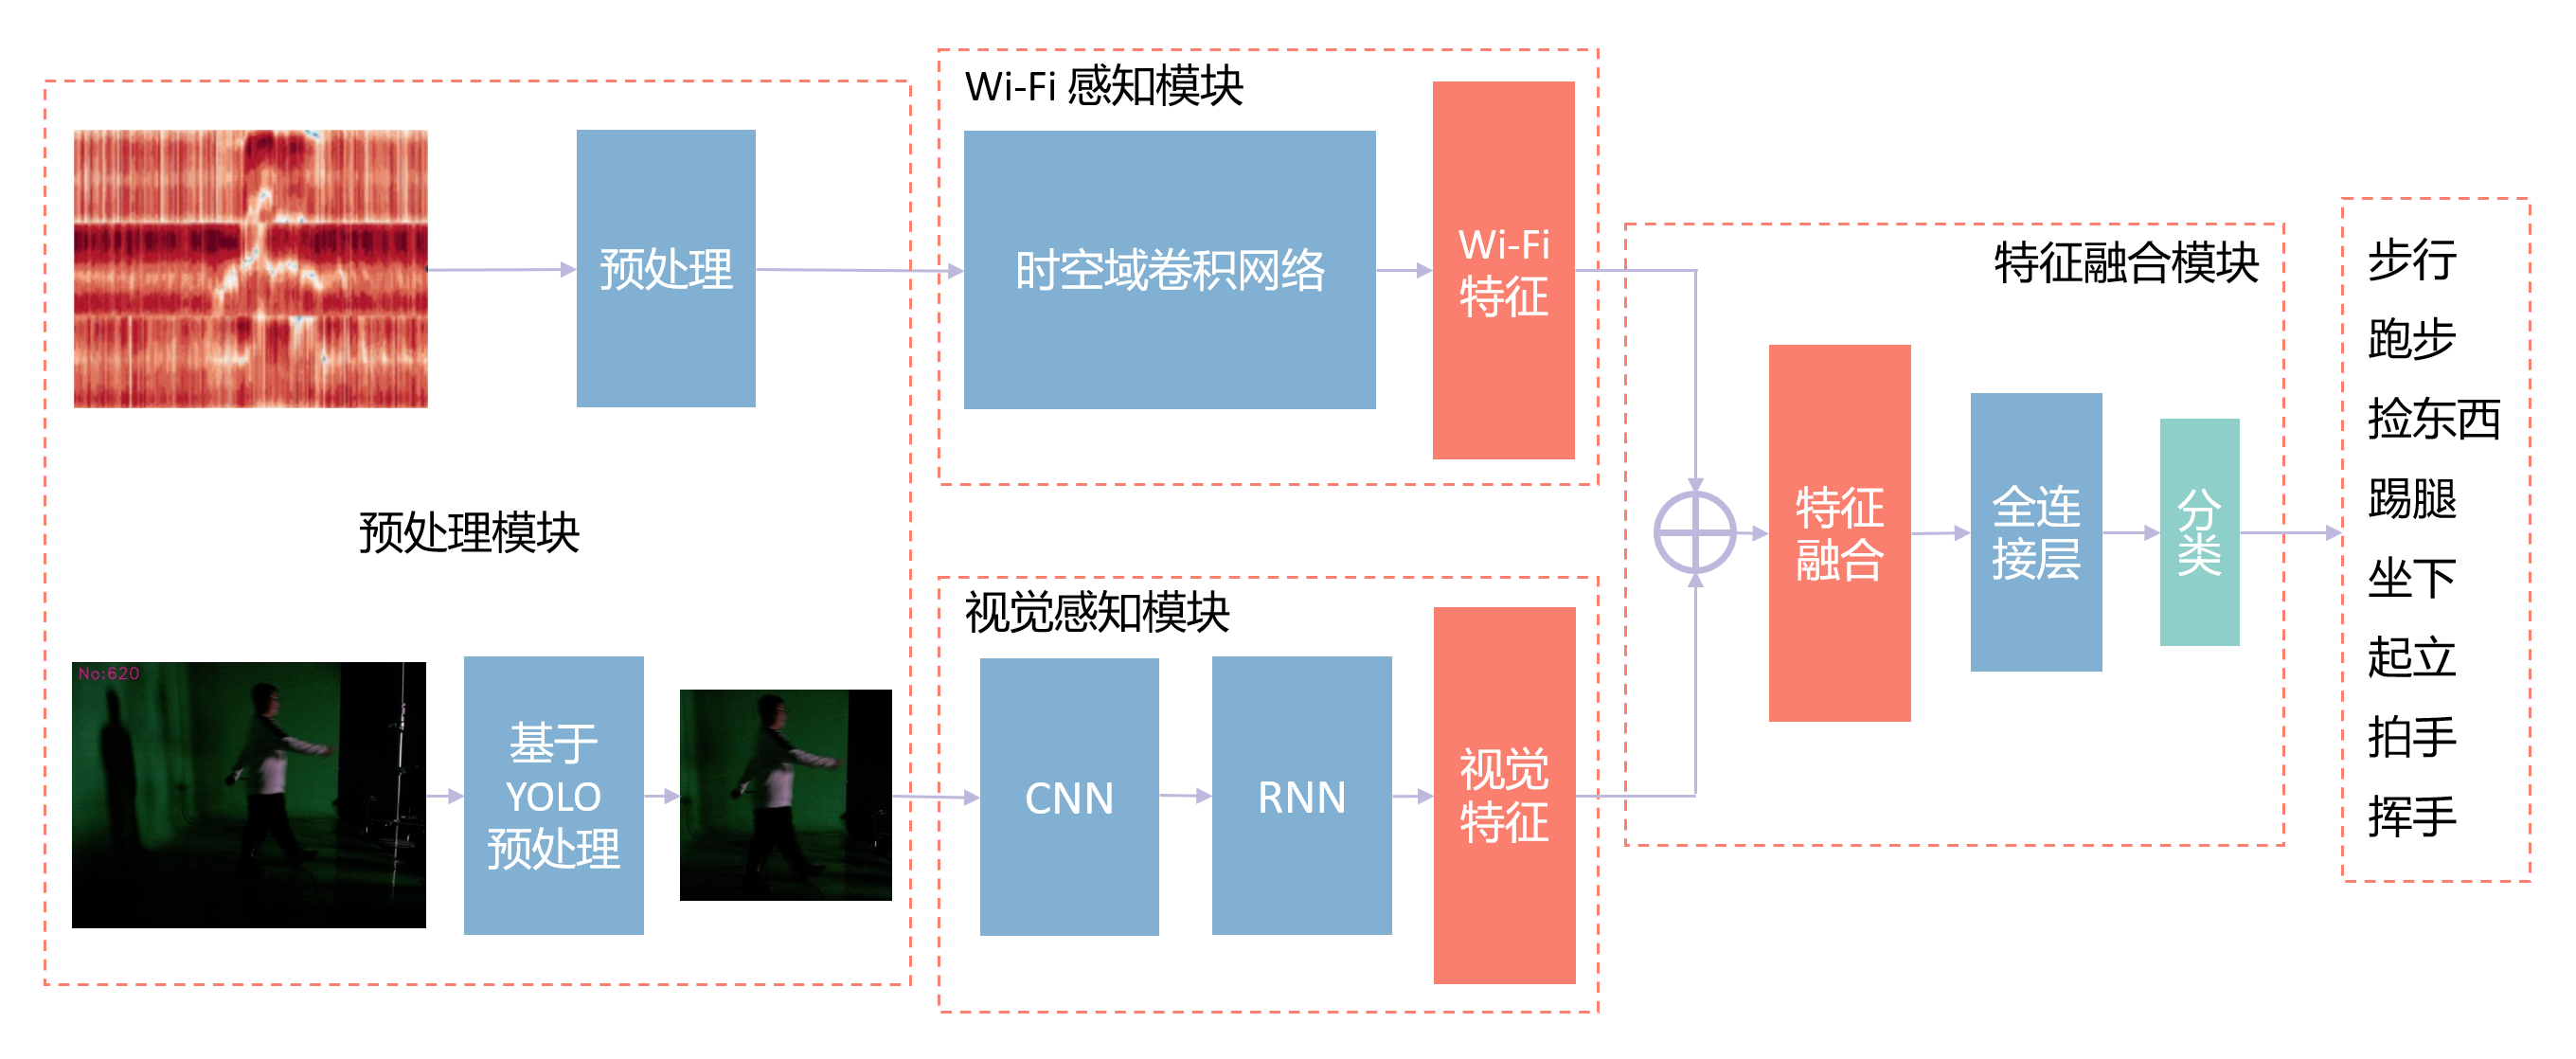
\includegraphics[scale = 0.165]{figures/system.png}
	\caption{\song\wuhao 模型系统架构示意图}
	\label{ViFi_system}
\end{figure}
\chapter{模型实现}
\label{chap04}
\defaultfont
\sloppy{}

\textbf{算法伪代码样例} \ref{YOLO}

% {\linespread{2.0}\selectfont
% \centerline{表4.1\quad\quad 基于 YOLO 进行视觉数据检测和裁剪预处理}
% }
\begin{algorithm}
% \caption{Video Data Preprocess by YOLO Detection and Cropping}
\caption{基于 YOLO 进行视觉数据检测和裁剪预处理}
\label{YOLO}
\begin{algorithmic}[1] % show line number
% \REQUIRE{$\mathcal{V}$ is data samples composed of video frames; $\mathcal{F}$ is the YOLO model; $acc$ is the confidence threshold for object recognition; $\mathcal{C} $ is the image cropping tool}
\REQUIRE{$\mathcal{V}$ 是视觉帧数据样例; $\mathcal{F}$ 是 YOLO 目标检测模型; $acc$ 物体的识别可信度; $\mathcal{C} $ 图片裁剪工具}
% \ENSURE{the detected person $\mathcal{P}$}
\ENSURE{被检测者 $\mathcal{P}$}

\FOR{each $\widetilde{v} \in \mathcal{V}$}
    \STATE $Z_i \gets \mathcal{F}(\widetilde{v})$
    \IF{$Z_i$ is not person and $Z_i^{acc} < acc$}
        \STATE discard
    \ENDIF
    \STATE expand the identified target $Z_i$ into a square $Z_i^{square}$
    \STATE $\mathcal{P} \gets \mathcal{C}(Z_i^{square})$
\ENDFOR
\end{algorithmic}
\end{algorithm}
% !TEX TS-program = XeLaTeX
% !TEX encoding = UTF-8 Unicode

\chapter{实验设计与结果分析}
\label{chap05}
\defaultfont
\sloppy{}

\textbf{表格样例} \ref{io_train_time_tab}

\begin{table}[htbp]
\setlength{\abovecaptionskip}{0cm}
% \setlength{\belowcaptionskip}{-0.2cm}
  \centering
  \song\wuhao
  \caption{A 和 B 模型时间开销(单位:秒)}
  \setlength{\tabcolsep}{3mm}{
    \begin{tabular}{ccccc}
    % \toprule
    \hline
    \multirow{2}[4]{*}{模型} & \multirow{2}[4]{*}{模态} & \multicolumn{3}{c}{任务} \\
\cmidrule{3-5}         & & epoch平均时长 & 输入输出处理用时 & 模型训练时长 \\
    % \midrule
    \hline
          & 视觉   & 37.3 & 33.0 & 4.3 \\
    CRNN  & Wi-Fi & 31.7 & 30.4 & 1.3 \\
          & 多模态 & 37.9 & 33.1 & 4.8 \\
    % \midrule
    \hline
          & 视觉   & 37.3 & 33.0 & 4.3 \\
    ViFi  & Wi-Fi & 32.5 & 30.5 & 2.0 \\
          & 多模态 & 38.8 & 33.5 & 5.3 \\ \hline
    % \bottomrule
    \end{tabular}}
  \label{io_train_time_tab}
\end{table}
% \include{body/chap06}
\cleardoublepage

% !TEX TS-program = XeLaTeX
% !TEX encoding = UTF-8 Unicode

\chapter*{\hfill 结  论 \hfill}
\addcontentsline{toc}{chapter}{结  论}
\label{conclusion}
\sloppy{}

简明扼要地回答研究问题:结论的首要目标是回答研究问题或验证研究假设。在结论部分,明确陈述你的研究问题,并提供对问题的回答或假设的验证结果。确保你的回答或验证是明确的,没有遗漏或模糊之处。

总结主要发现:总结你的研究中的主要发现和结果。列出你的研究结果,并将其归纳为几个主要观点或主题。确保提及每个主要发现,并指出其对研究问题的重要性和贡献。

讨论研究结果:在结论部分,可以对你的研究结果进行进一步的讨论。解释结果的意义和影响,以及与现有研究或理论的关联。探讨结果可能的解释、局限性和不确定性,并提出进一步研究的建议。

强调研究的重要性:在结论部分,再次强调你的研究的重要性和独特性。说明你的研究对学术界、实践领域或社会的意义和影响。指出你的研究填补了现有知识的空白或为进一步研究提供了基础。

提出建议或展望未来研究:根据你的研究结果,提出未来研究的建议或展望。指出你的研究可能存在的局限性,并提出进一步深入研究的方向。这样可以为其他研究者提供有关如何扩展你的研究的指导。

结论的凝练和清晰:结论部分应该简明扼要,避免冗长和重复。用清晰、简练的语言表达你的结论,并确保其与论文的整体内容保持一致。

结论是理论分析和实验结果的逻辑发展,是整篇论文的归宿。结论是在理论分析、试验结果的基础上,经过分析、推理、判断、归纳的过程而形成的总观点。结论必须完整、准确、鲜明、并突出与前人不同的新见解。

书写格式说明:

标题“结论”选用模板中的样式所定义的“结论”,或者手动设置成字体:黑体,居中,字号:小三,1.5倍行距,段后1行,段前为0行。

结论正文选用模板中的样式所定义的“正文”,每段落首行缩进2字;或者手动设置成每段落首行缩进2字,字体:宋体,字号:小四,行距:多倍行距 1.25,间距:段前、段后均为0行。
\song\wuhao
\setmainfont{SIMSUN.TTC}
\linespread{1.25}
% \setlist[enumerate]{[1],itemsep=-3pt,topsep=0mm,labelindent=\parindent,leftmargin=*}
% \chapter*{\hfill 参~考~文~献 \hfill}
\addcontentsline{toc}{chapter}{参~考~文~献}
\label{reference}
\sloppy{}

参考文献推荐使用bibtex或bibitem生成,如有需要可自行补充填写bibtex。另需注意,如果引用了硕士/博士毕业论文,需要添加城市信息,可参考reference.bib

% \begin{thebibliography}{99}
% \bibitem{khurana2018deep}Khurana R, Kushwaha A K S. Deep learning approaches for human activity recognition in video surveillance-a survey[C]//2018 First International Conference on Secure Cyber Computing and Communication (ICSCCC). IEEE, 2018: 542-544.
% \bibitem{baccouche2011sequential}Baccouche M, Mamalet F, Wolf C, et al. Sequential deep learning for human action recognition[C]//Human Behavior Understanding: Second International Workshop, HBU 2011, Amsterdam, The Netherlands, November 16, 2011. Proceedings 2. Springer Berlin Heidelberg, 2011: 29-39.
% \end{thebibliography}
% \vspace{17.06pt}

% 标题“参考文献”不可省略,选用模板中的样式所定义的“参考文献”;或者手动设置成字体:黑体,居中,字号:小三,1.5倍行距,段后1行,段前为0行。

% 参考文献内容设置成字体:宋体,字号:五号,多倍行距1.25,段前、段后均为0行,取消网格对齐选项。

% 参考文献的著录,按论文中引用顺序排列。

% 参考文献数量不少于10篇,其中期刊不少于5篇,并且包含一定数量的外文期刊。

% 文献类型标志参考国家标准 GB/T 7714-2005,如下表:

\vspace{17.06pt}
\bibliography{reference}


\setmainfont[Mapping=tex-text]{Times New Roman}
% !TEX TS-program = XeLaTeX
% !TEX encoding = UTF-8 Unicode

\chapter*{\hfill 附录A\quad 附录内容名称 \hfill}
\addcontentsline{toc}{chapter}{附录A\quad 附录内容名称}
\defaultfont
\linespread{1.25}
\sloppy{}

以下内容可放在附录之内:

(1) 正文内过于冗长的公式推导;

(2) 方便他人阅读所需的辅助性数学工具或表格;

(3) 重复性数据和图表;

(4) 论文使用的主要符号的意义和单位;

(5) 程序说明和程序全文;

(6) 调研报告;

(7) 翻译部分有关说明。

这部分内容可省略。如果省略,删掉此页。

书写格式说明:

标题“附录A 附录内容名称”选用模板中的样式所定义的“附录”;或者手动设置成字体:黑体,居中,字号:小三,1.5倍行距,段后1行,段前为0行。

附录正文选用模板中的样式所定义的“正文”,每段落首行缩进2字;或者手动设置成每段落首行缩进2字,字体:宋体,字号:小四,行距:多倍行距 1.25,间距:段前、段后均为0行。

% !TEX TS-program = XeLaTeX
% !TEX encoding = UTF-8 Unicode

\chapter*{\hfill 修改记录 \hfill}
\addcontentsline{toc}{chapter}{修改记录}
\defaultfont
\linespread{1.25}
\sloppy{}

修改是论文写作过程中不可或缺的重要步骤,是提高论文质量的有效环节。修改的过程其实就是“去伪存真”、去糟粕取精华使论文不断“升华”的过程。

以下内容要求放到毕业设计(论文)修改记录中:

一、毕业设计(论文)题目修改

原题目:基于快速组网验证算法的优化算法

修稿后题目:基于 WiFi 和视觉的多模态行为识别方法研究

二、毕业设计(论文)内容重要修改记录

{\textbf {第一次修改记录:}}:

括号格式,修改前:中英文括号混用。

{\textbf{修改后:}}全部使用中文括号,在第一次出现的专有名词缩写后添加详细解释。

{\textbf {第二次修改记录:}}:

论文格式,修改前:列表换行没有顶头,公式变量没有统一。

{\textbf{修改后:}}修改列表格式,使用标准字母大小,全文统一变量指代内容,图标添加标注。

{\textbf {第三次修改记录:}}:

摘要和结论,修改前:内容较为混乱。

{\textbf{修改后:}}重写了摘要和结论部分,强调重要性和系统设计。

三、毕业设计(论文)外文翻译修改记录

四、毕业设计(论文)正式检测重复比

\hspace*{7.8cm}记录人(签字):\\
\hspace*{8.2cm}指导教师(签字):
% !TEX TS-program = XeLaTeX
% !TEX encoding = UTF-8 Unicode

\chapter*{\hfill 致  谢 \hfill}
\addcontentsline{toc}{chapter}{致  谢}
\defaultfont
\linespread{1.25}
\sloppy{}

毕业设计(论文)致谢中不得书写与毕业设计(论文)工作无关的人和事,对指导老师的致谢要实事求是。

对其他在本研究工作中提出建议和给予帮助的老师和同学,应在论文中做明确的说明并表示谢意。

这部分内容不可省略。

书写格式说明:

标题“致谢”选用模板中的样式所定义的“致谢”;或者手动设置成字体:黑体,居中,字号:小三,1.5倍行距,段后1行,段前为0行。

致谢正文选用模板中的样式所定义的“正文”,每段落首行缩进2字;或者手动设置成每段落首行缩进2字,字体:宋体,字号:小四,行距:多倍行距 1.25,间距:段前、段后均为0行。

% 使用时将此处删掉即可
% !TEX TS-program = XeLaTeX
% !TEX encoding = UTF-8 Unicode

\chapter*{\hfill 作  者 \hfill}
\defaultfont
\linespread{1.25}
\sloppy{}

为及时发现模板中存在的问题,在此处给出各位作者的联系方式,欢迎大家积极反馈。在正式使用时请将此页删除。\\

模板原作者:

\vspace{17.06pt}
\textbf{指导教师:} 王洁${(\textrm{\Letter}}$ \href{mailto:wang_jie@dlut.edu.cn}{wang\_jie@dlut.edu.cn)}

\vspace{17.06pt}
\textbf{学生:} 赵小棠 ${(\textrm{\Letter}}$ \href{mailto:xiaotang_zhao@outlook.com}{xiaotang\_zhao@outlook.com)}

\vspace{17.06pt}
\textbf{学生:} 李鹏飞 ${(\textrm{\Letter}}$ \href{mailto:1468735412@qq.com}{1468735412@qq.com)}

\vspace{17.06pt}
\textbf{学生:} 吴鑫涛 ${(\textrm{\Letter}}$ \href{mailto:614344805@qq.com}{614344805@qq.com)}\\

修改作者:

\vspace{17.06pt}
\textbf{2023届毕业生:} Augists ${(\textrm{\Letter}}$ \href{mailto:augists@duck.com}{augists@duck.com)}

\backmatter

\end{document}
